\chapter{Graphs and Networks}


\section{Heavily Labeled Citation Graph}\label{appendix:fullauthor}

\begin{figure}[H]
     \centering
         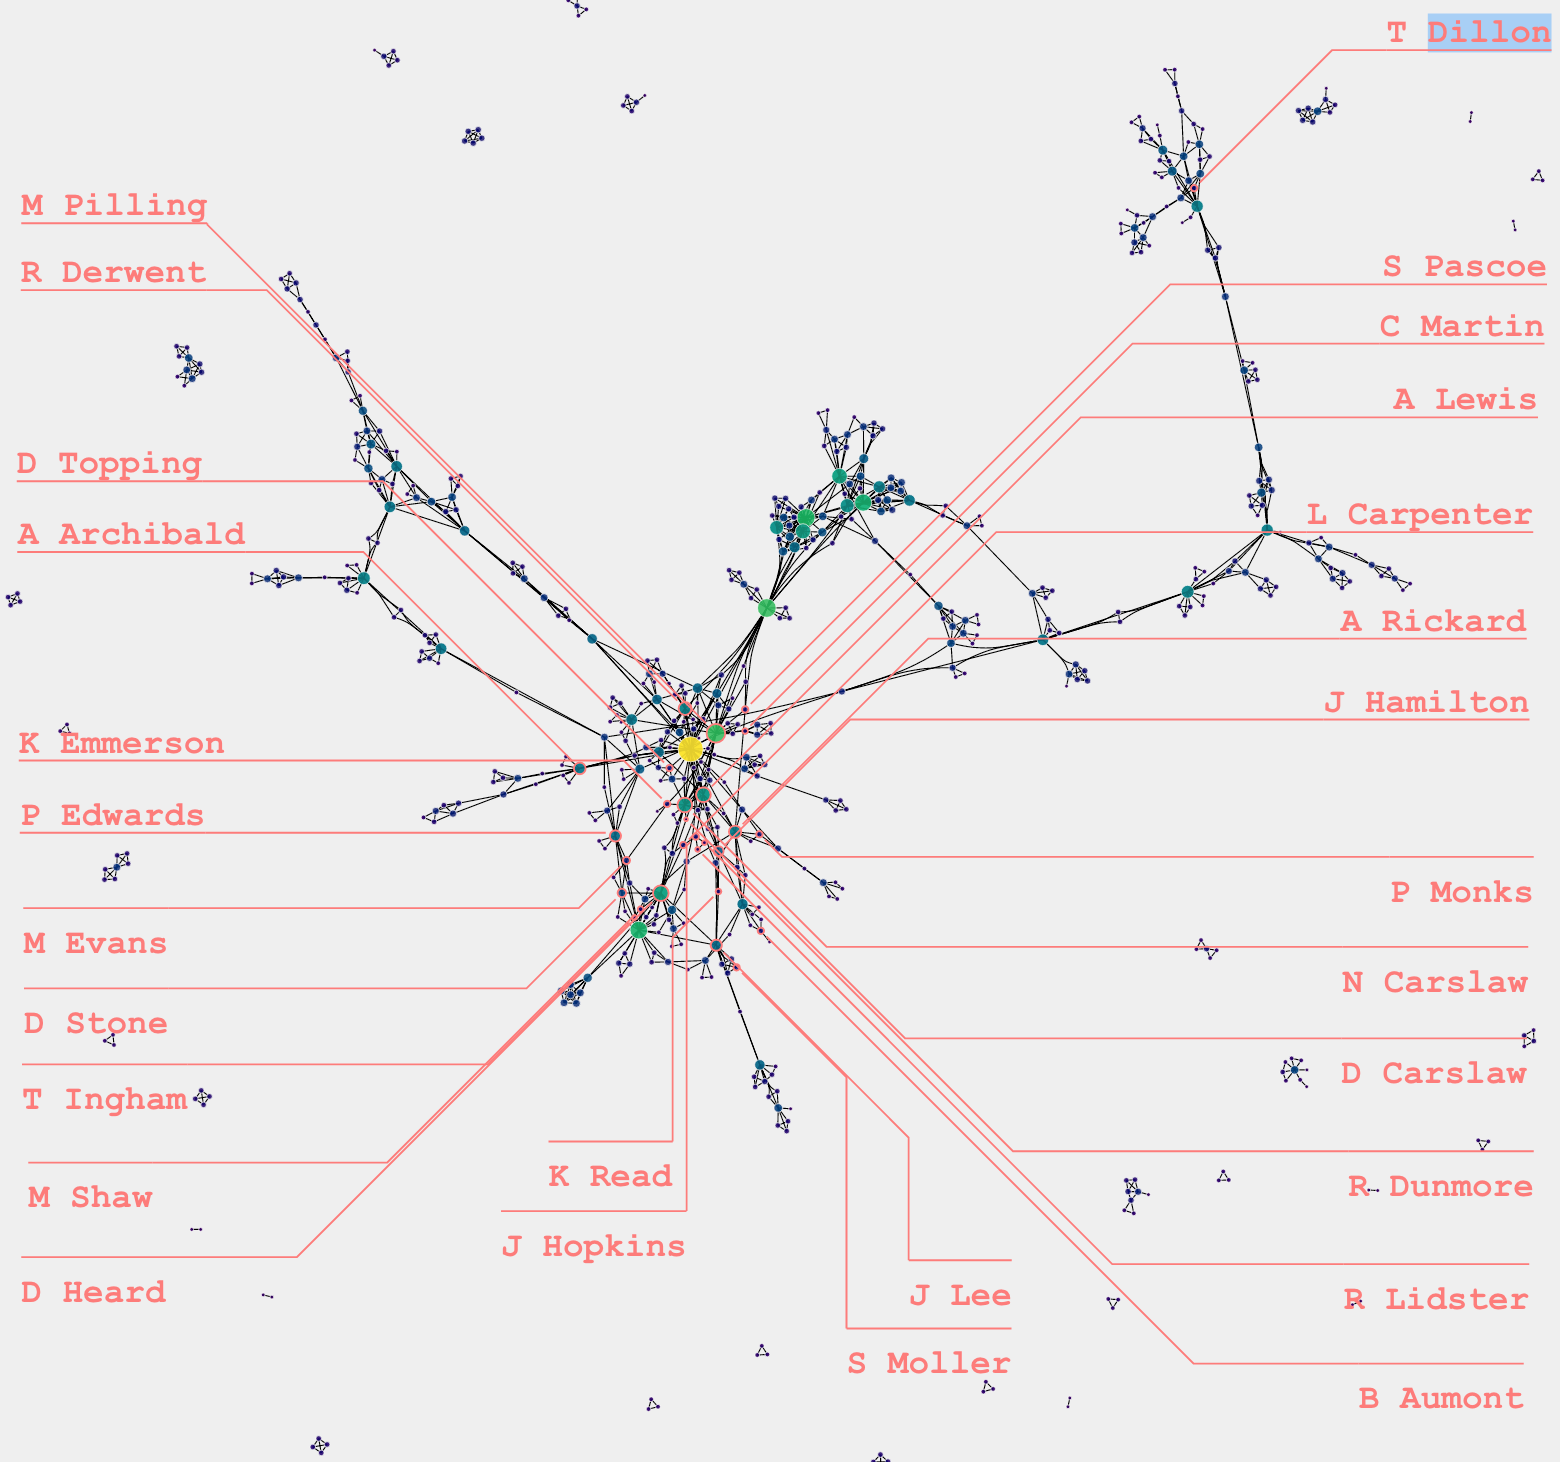
\includegraphics[width=\textwidth]{WACLauthor.png}
        \caption{ \textbf{The labelled co-author network -} as  referenced in \autoref{ch3} }

\end{figure}
\newpage


\section{Centrality on the UK rail network.}\label{appendix:rail}

The data in the following section was extracted from OpenStreetData using overpass turbo \url{https://overpass-turbo.eu}. Here ways within the geographic information system mapping (GIS) format are represented as paths between locations (i.e. a graph). Following some simple processing, the distance of each section was calculated, and a weighted graph represented the UK rail network was generated. This was then used to form a rudimentary analysis of the graph structure using centrality metrics (shown below).

\textbf{NOTE:}\\
\textit{Since the network is extracted from a GIS data file, nodes within the rail network include not only stations but also switches, routing nodes and crossings. Although this can be filtered, the iterative reconstruction of a graph for the entire UK is a lengthy process - one which I am unable to do at the time of writing (there are 90011 nodes which make up the entirety of the UK rail network, most of which need to be removed, and their links rerouted).}


\begin{figure}[H]
     \centering
\begin{subfigure}[b]{.49\textwidth}
     \centering
         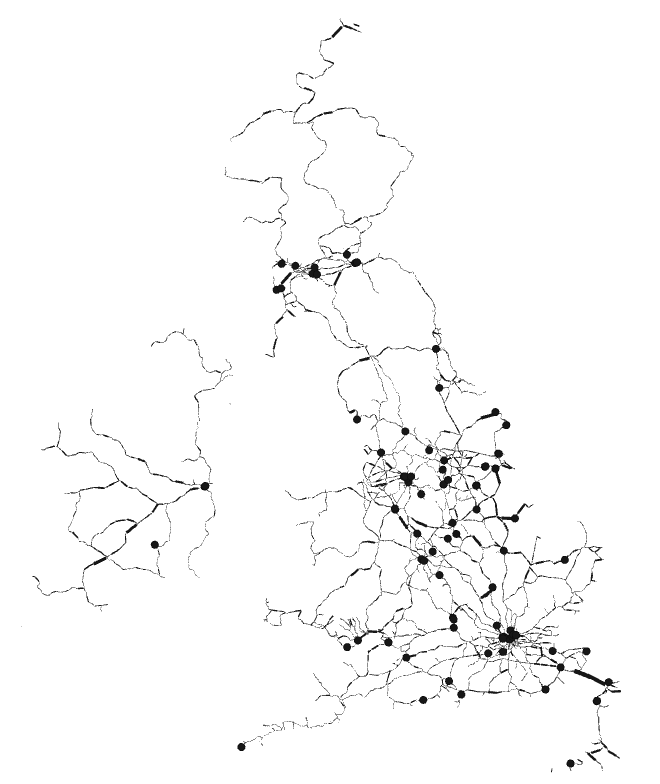
\includegraphics[width=\textwidth]{rail/degree.png}
        \caption{ \textbf{Degree Centrality.}}
\end{subfigure}
\begin{subfigure}[b]{.49\textwidth}
     \centering
         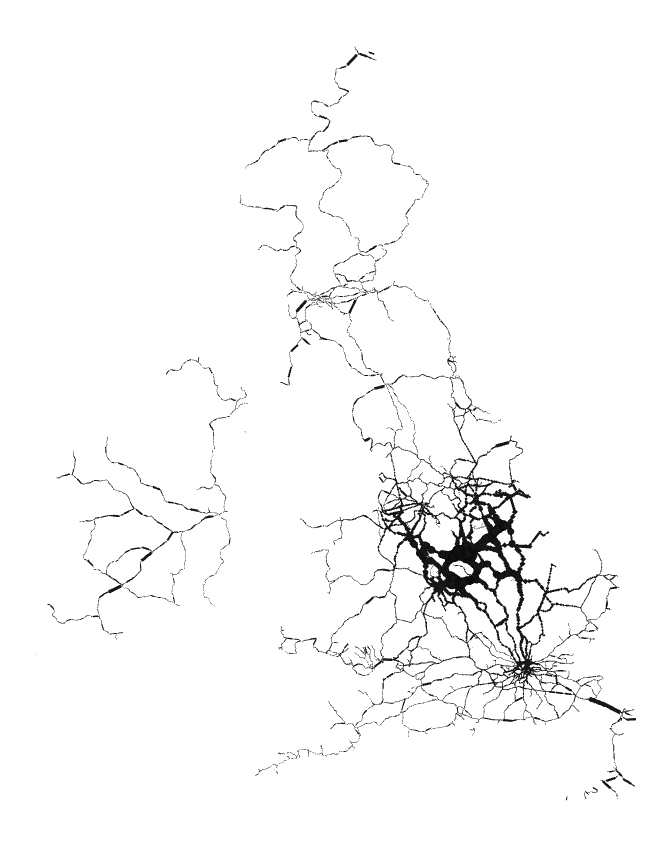
\includegraphics[width=\textwidth]{rail/centrality.png}
        \caption{ \textbf{Closeness Centrality.}}
\end{subfigure}

\begin{subfigure}[t]{.49\textwidth}
     \centering
         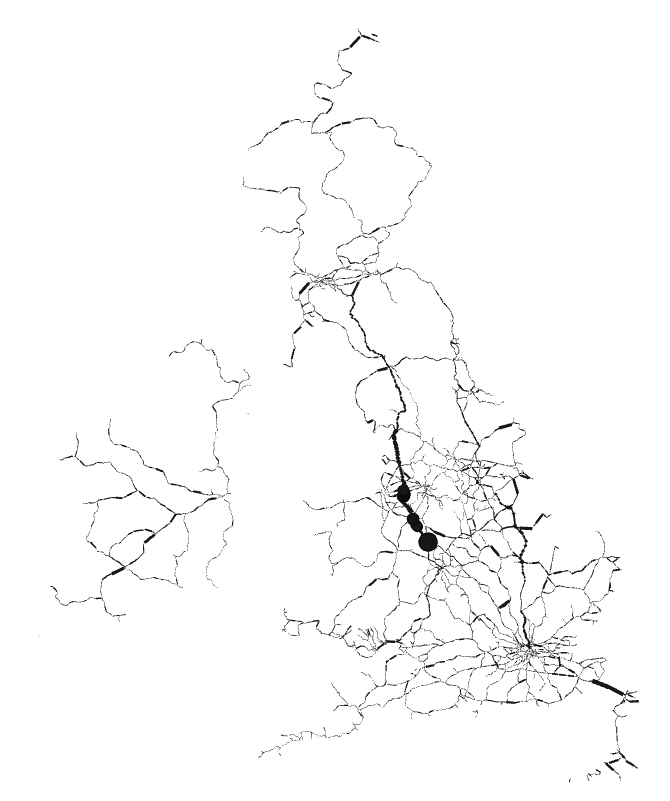
\includegraphics[width=\textwidth]{rail/betweenness.png}
        \caption{ \textbf{Betweenness Centrality.}}
\end{subfigure}
\begin{subfigure}[t]{.49\textwidth}
     \centering
          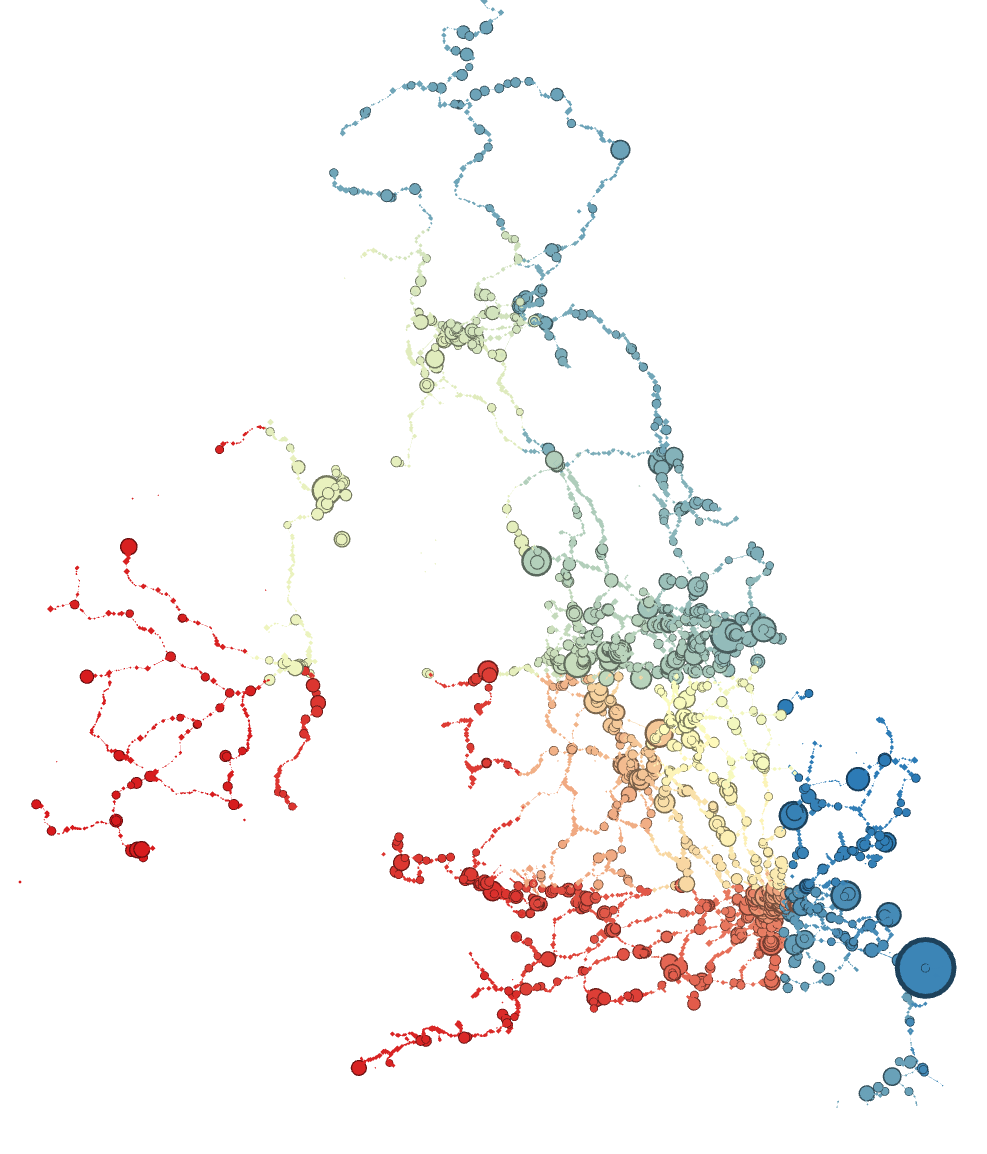
\includegraphics[width=\textwidth]{rail/pagerank.png}
        \caption{ \textbf{PageRank Centrality.} Colours are groups from the modularity clustering algorithm which partitions the network into highly connected areas or `cliques'.}
\end{subfigure}
\end{figure}







\chapter{Miscellaneous}




\section{Correspondence with Mike Jenkin}\label{appendix:correspondance}
Mike Jenkin 11th September 2019

\textbf{Note on naming conventions in the CRI mechanism}\\

{\fontfamily{cmtt}\selectfont \parbox{\textwidth}{
The lumped or “common” species in the CRI mechanism are, by definition, used to represent a set of real species with different structures and properties. The criterion for lumping is the maximum number of NO-to-NO2 conversions (i.e. maximum number of ozone molecules) that the subsequent degradation can produce - and lumped species can, therefore, represent a large number of real species with different structures and properties.
\\}\\ \parbox{\textwidth}{
In later expansions of the mechanism, the chemistry for species such as isoprene and terpenes defined intermediates that are representative of more restricted sets of real species. For these, it is possible to relate them to more restricted sets of MCM species that are the main contributors.
\\}\\ \parbox{\textwidth}{
Although I tried to be logical in naming, the mechanism was developed over many years with little or no funding and may therefore not be fully transparent and foolproof throughout. However, I think quite a lot of the naming is logical, as expanded on below.
\\}\\ \parbox{\textwidth}{
1) The numbers in most of the species names (the “CRI index”) are the number of NO-to-NO2 conversions that can result from the subsequent OH-initiated NO-propagated chemistry. For radical termination products (e.g. hydroperoxides formed from RO2 + HO2 and nitrates formed from RO2 + NO), this is a grey area, and the number is, therefore, the same as that for the precursor RO2 radical. In these cases, it is simply a convenient label.
\\}\\ \parbox{\textwidth}{
2) There are a number of series of peroxy radicals, which are denoted RNxxO2, RIxxO2, RAxxO2, RExxO2, RUxxO2, RTNxxO2, RTXxxO2. These represent peroxy radicals with different structural features or formed from different types of precursor, as indicated below. Occasionally, extra peroxy radicals with the same CRI index are included by inserting a letter after the index (e.g. RNxxAO2) to increase flexibility of the mechanism. Peroxy radicals formed specifically from addition of NO3 to an alkene/diene are prefixed by “N”.
\\}\\ \parbox{\textwidth}{
RNxxO2: These were originally representative of peroxy radicals formed from linear or “n-“ alkanes and their carbonyl products. They are also used for peroxy radicals formed from slightly-branched precursors (e.g. 2-methylhexane), and are formed as a convenient default intermediate with the correct CRI index in the latter stages of degradation of other precursor classes.
\\}\\ \parbox{\textwidth}{
RIxxO2: These were originally representative of peroxy radicals formed from branched or “i-“ alkanes and their carbonyl products, but tend to be used only for smaller branched precursors that can produce acetone as a major product from their subsequent degradation. This is because acetone is a particularly unreactive carbonyl, the formation of which can interrupt the ozone formation processes under typical regional-scale photochemical episode conditions in north-west Europe.
\\}\\ \parbox{\textwidth}{
RAxxO2: These peroxy radicals are formed from the addition of OH to aromatic compounds, and are complex bicyclic structures containing a peroxide bridge (e.g. like BZBIPERO2 in the MCM).
\\}\\ \parbox{\textwidth}{
RExxO2: These peroxy radicals are formed from ether degradation, and allow the formation of unreactive formate ester products to be represented.
\\}\\ \parbox{\textwidth}{
RUxxO2: These peroxy radicals are formed from degradation of conjugated dienes (currently only isoprene and 1,3-butadiene). Those formed initially (e.g. RU14O2) contain allyl functionalities (i.e. a specific unsaturated linkage), although the terminology is also used for some peroxy radicals formed from subsequently-formed unsaturated products.
\\}\\ \parbox{\textwidth}{
Related to this, the species CRU14O2 and TRU14O2 in the EMEP variant of CRI v2.2 (described in \url{https://doi.org/10.1016/j.atmosenv.2019.05.055}) were specifically introduced to represent the cis- and trans- isomers required for the Peeters (LIM) reaction framework. CRU14O2 represents CISOPAO2 and CISOPCO2 in MCM v3.3.1 and TRU14O2 represents ISOPAO2 and ISOPCO2 in MCM v3.3.1. However, CRI v2.2 itself uses a different approach where the chemistry is represented by a conditions-dependent rate coefficient for the single peroxy radical, RU14O2.
\\}\\ \parbox{\textwidth}{
RTNxxO2: This terminology is used for peroxy radicals formed from monoterpenes containing an endocyclic double bond. This is currently limited to $\alpha$-pinene in CRI, although the original idea was that the mechanism could be used as a surrogate for other endocyclic monoterpenes by simply adding new sets of initiation reactions.
\\}\\ \parbox{\textwidth}{
RTXxxO2: This terminology is used for peroxy radicals formed from monoterpenes containing an exocyclic double bond. This is currently limited to $\beta$-pinene in CRI, although the original idea was that the mechanism could be used as a surrogate for other exocyclic monoterpenes by simply adding new sets of initiation reactions.
\\}\\ \parbox{\textwidth}{
Finally, the species DHPR12O2 in CRI v2.2 is a peroxy radical containing two hydroperoxy groups. Again, it is required for representation of the Peeters (LIM) mechanism, and is representative of the species C536O2 and C537O2 in MCM v3.3.1 (these species being referred to as “di-HPCARPs” by Peeters et al., 2014: \url{https://doi.org/10.1021/jp5033146}).
\\}\\ \parbox{\textwidth}{
3) Hydroperoxides formed the reactions of HO2 with the above peroxy radicals have “OOH” in place of “O2”. Nitrates formed the reactions of NO with the above peroxy radicals have “NO3” in place of “O2”.
\\}\\ \parbox{\textwidth}{
4) There are a number of series of carbonyl compounds, which are denoted CARBxx, UCARBxx, UDCARBxx, TNCARBxx and TXCARBxx.
\\}\\ \parbox{\textwidth}{
CARBxx: These are used to represent carbonyls and hydroxycarbonyls. Occasionally, extra carbonyls/hydroxycarbonyls with the same CRI index are included by inserting a letter after the index (e.g. CARBxxA) to increase the flexibility of the mechanism.
\\}\\ \parbox{\textwidth}{
Related to this, the species DHPCARB9 in CRI v2.2 is a carbonyl containing two hydroperoxy groups. Again, it is required for representation of the Peeters (LIM) mechanism, and is representative of the species DHPMEK and DHPMPAL in MCM v3.3.1  in MCM v3.3.1.
\\}\\ \parbox{\textwidth}{
UCARBxx: This terminology is used for unsaturated carbonyls/hydroxycarbonyls, formed for example from isoprene (although one of the main ones, UCARB10, has been “unlumped” into MVK and MACR in the EMEP CRI v2.2 variant).
\\}\\ \parbox{\textwidth}{
Related to this, the species HPUCARB12 in CRI v2.2 is an unsaturated carbonyl containing a hydroperoxy group. Again, it is required for representation of the Peeters (LIM) mechanism, and is representative of the species C5HPALD1 and C5HPALD2 in MCM v3.3.1.
\\}\\ \parbox{\textwidth}{
UDCARBxx: This terminology is used for unsaturated dicarbonyls, formed from aromatics.
\\}\\ \parbox{\textwidth}{
TNCARBxx and TXCARBxx: This terminology is used for carbonyl compounds, formed from monoterpenes with endocyclic and exocyclic double bonds, respectively.

}}



\section{Functional Groups}\label{appendix:fngroups}
\begin{figure}[H]
\centering
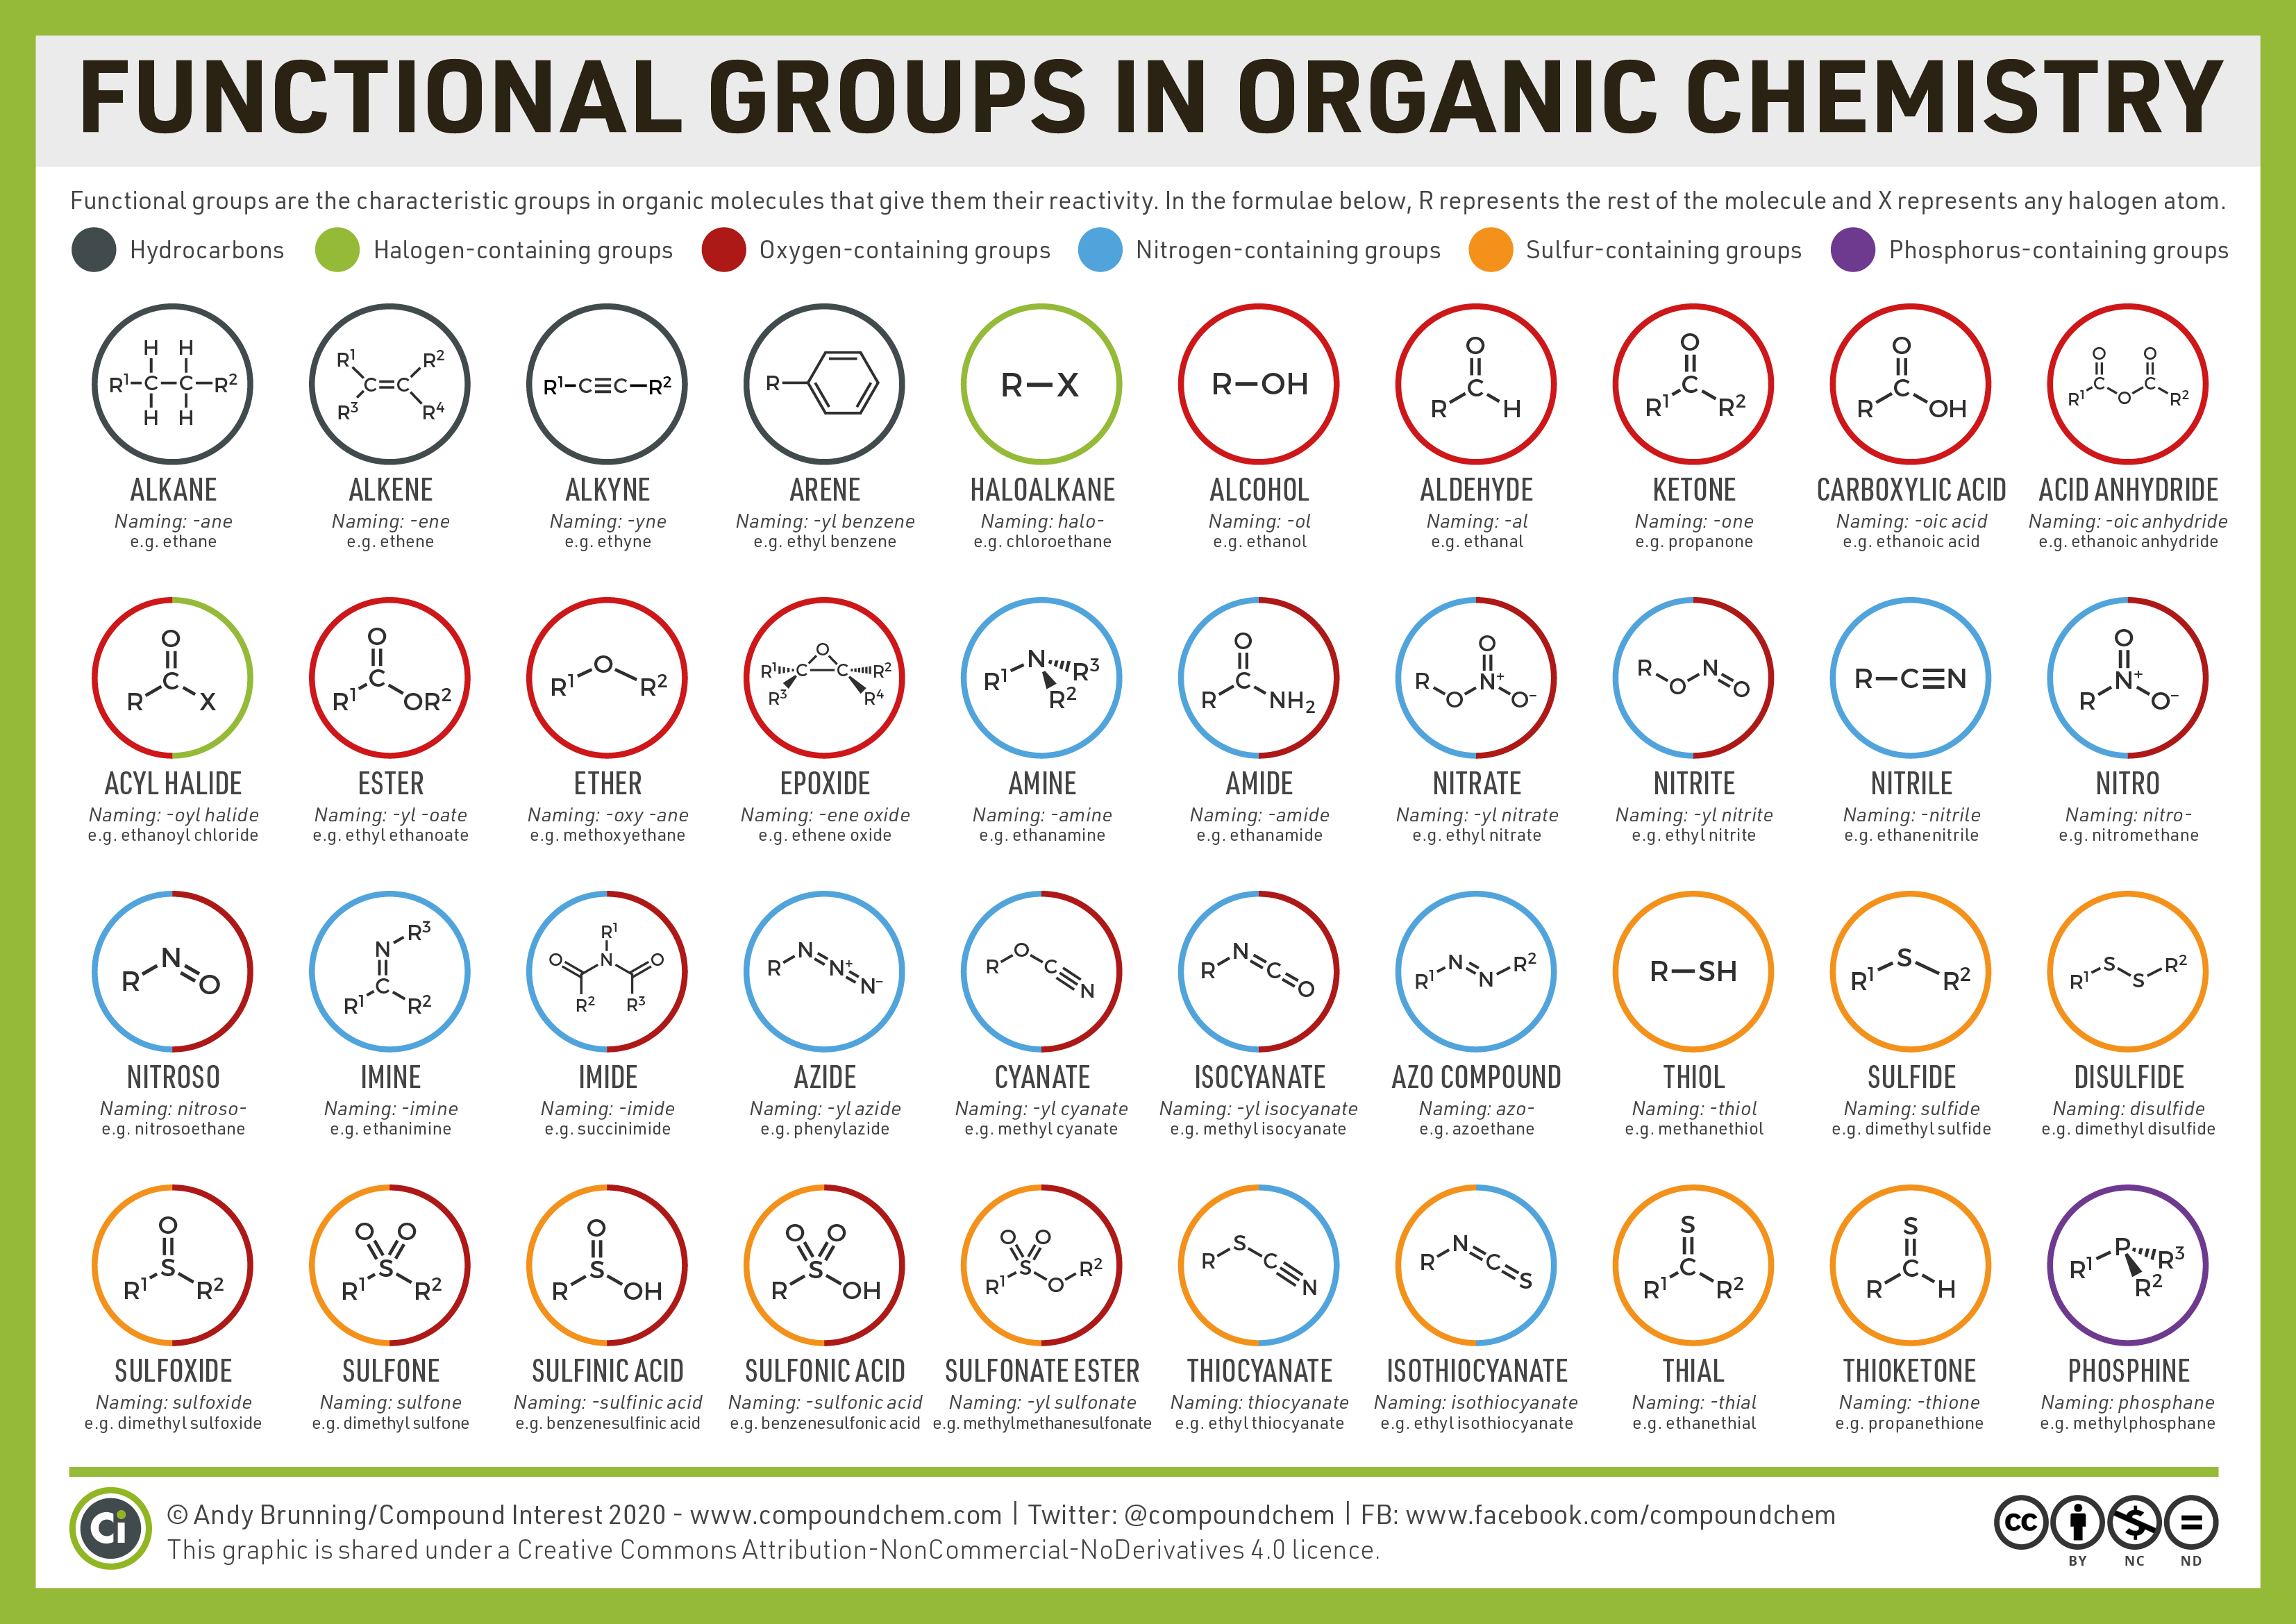
\includegraphics[width=.9\textheight,angle=90]{fngroups.png}
{}
\end{figure}
